\documentclass[12 pt]{exam}
\usepackage[margin=0.75in]{geometry}
\usepackage{amsmath,amssymb,color,amsthm}
\usepackage{enumerate,graphicx,multicol}
\usepackage{wrapfig}
\usepackage{pgf,tikz, subcaption, hyperref}
\usetikzlibrary{arrows}

\printanswers

\newtheorem{claim}{Claim}
\newtheorem{lemma}{Lemma}

\pagestyle{head}                       % This causes the exam to only have headers, no footers.
%\runningheadrule                     % This causes the headings to have an underline.

%\firstpageheader{Name:\enspace\hbox to 4.5in{\hrulefill} Section:\enspace\hbox to 1.2in{\hrulefill}}{}{}
%\extraheadheight{.25in}

\begin{document}
\hrule
\begin{center}
  \huge{Math 2710 Problem Set 10: Ch 3}    %Title
\end{center}
\hrule
\vskip .2in

\begin{questions}
%% Add some harder counting questions from the eariler sections!!
\question You are trying to decide on a one topping pizza. You have three options for crust - thin, original or thick, two options for sauce (red and white) and 5 choices of toppings. 
\begin{parts}
\part Without using the multiplication principle, describe how you would find the total number of possible pizzas you could make. 

\begin{solution}
Draw a tree diagram, branching out on every crust, sauce, and topping choice, and count the number of pizzas
on the right side.
\end{solution}


\part Explain how to use the multiplication principle in the context of this problem. 

\begin{solution}
Possible pizzas = 3 crusts * 2 sauces * 5 toppings = 30 total pizzas.
\end{solution}


\part Explain why the multiplication principle works. 

\begin{solution}
Because every having n choices at any decision point means that you have n times
the number of outcomes as before.
\end{solution}


\end{parts}

\question The US Government wants to assign each person in the US a passcode, which is a string of lowercase letters. How many letters should they use so that there are enough different passcodes for each person to have one? Explain how you went about solving this problem. 

\begin{solution}
\# passcodes for a n-length string of lowercase letters = $26^n$.

US population is 340 million. Then,

\begin{align*}
    340 \cdot 10^6 &\ge 26^n\\
    \log_{26}(340 \cdot 10^6) &\ge n\\
    6.029 \ge n\\
\end{align*}

So we need to use a $7$-letter passcode.
\end{solution}


\question  How many different Chipotle Burrito options are there \url{https://www.chipotle.com/content/dam/poc/order/nutrition-files/PaperMenu_STANDARD_NoPricing_120221_us.pdf}? (Answers may vary, you can decide if you are allowed to choose multiple things in each category.)

\begin{solution}
Meats: 6

Toppings: $2^{14}$

Total: $6 * 2^{14}$
\end{solution}



\question Six math books, four physics books and three chemistry books are arranged on
a shelf. How many arrangements are possible if all books of the same subject
are grouped together?

\begin{solution}\\
Math book permutations: $6!$

Physics book permutations: $4!$

Chemistry book permutations: $3!$

Then you have $3!$ ways to arrange math, physics, and chemistry.

So $6! \cdot 4! \cdot 3! \cdot 3!$.
\end{solution}


\question How many 4-permutations are there of the set $\{A,B,C,D,E,F\}$if whenever $A$
appears in the permutation, it is followed by $E$?

\begin{solution}\\
No A: then 4-permutations of $\{B, C, D, E, F\}$, so $5(4)(3)(2)$.

1 AE: then 2-permutations are $\{B, C, D, F\}$, so $4(3)$.
You can have AExx or xxAE or xAEx, so 3 ways to arrange AE and the 2 letters, so $4(3)(3) = 36$.

Alt: choose 2 letters in $\{B, C, D, F\}$, then 3! ways to arrange AE and 2 letters,
so $\binom{4}{2} 3! = \frac{4!}{2!(4-2)!} 3! = 2(3) 3! = 36$

Total: $5(4)(3)(2) + 4(3)(3) = 156$.
\end{solution}


\question  A department consists of 5 men and 7 women. From this department you select
a committee with 3 men and 2 women. In how many ways can you do this?

\begin{solution}\\
$\binom{5}{3}$ to choose 3 men from 5. $\binom{7}{2}$ ways to choose 2 women from 7 women.

So $\binom{5}{3} \cdot \binom{7}{2} = 210$.
\end{solution}



\question Use the binomial theorem to find the coefficient of $x^{10}$ in $(x+2)^{15}.$

\begin{solution}
$\binom{15}{5} * 2^5 = 96096$
\end{solution}



\question Consider the expression $\sum_{k=0}^n 9^k \binom{n}{k}$. Evaluate the sum for several small values of $n$ and make a conjecture. Then prove that using the binomial theorem.

\begin{solution}\\
$n=0: 9^0 \binom{0}{0} = 1$

$n=1: 9^0 \binom{1}{0} + 9^1 \binom{1}{1} = 1 + 9 = 10$

$n=2: 9^0 \binom{2}{0} + 9^1 \binom{2}{1} + 9^2 \binom{2}{2} = 1 + 18 + 81 = 100$\\

Conjecture: $\sum_{k=0}^n 9^k \binom{n}{k} = 10^n$

\begin{proof}
\begin{align*}
    \sum_{k=0}^n 9^k \binom{n}{k} &= (1+9)^n \qquad \text{by the Binomial Theorem}\\
    &= 10^n
\end{align*}
\end{proof}
\end{solution}



\question Show, via induction, that $\sum_{k=0}^n \binom{k}{r} = \binom{n+1}{r+1},$ where $1 \leq r \leq n$. 

\begin{solution}\begin{proof}
We proceed by induction.\\

Base case $n=1$: $1 \le r \le 1$, so $r = 1$

$\sum_{k=0}^n \binom{k}{r} = \binom{0}{1} + \binom{1}{1} = 0 + 1 = 1$

$\binom{2}{2} = 1$

So $\sum_{k=0}^n \binom{k}{r} = \binom{n+1}{r+1}$ for $n=1$.\\

Induction step: Assume that $\sum_{k=0}^n \binom{k}{r} = \binom{n+1}{r+1}$.

\begin{align*}
    \sum_{k=0}^i \binom{k}{r} &= \binom{i+1}{r+1}\\
    \sum_{k=0}^i \binom{k}{r} + \binom{i+1}{r} &= \binom{i+1}{r+1} + \binom{i+1}{r}\\
    \sum_{k=0}^{i+1} \binom{k}{r} &= \binom{i+2}{r+1}\\
\end{align*}

Then by induction we have that $\sum_{k=0}^n \binom{k}{r} = \binom{n+1}{r+1}$.
\end{proof}\end{solution}



\question Show, via induction, that $\sum_{k=0}^p \binom{m}{k}\binom{n}{p-k} = \binom{m+n}{p},$ where $m,n$ and $p$ are non-negative integers. 

\begin{solution}\begin{proof}
We proceed by induction.\\

Base case $n=0$:
\begin{align*}
    \sum_{k=0}^p \binom{m}{k} \binom{n}{p-k} &= \sum_{k=0}^p \binom{m}{k} \binom{0}{p-k}
    = \sum_{k=0}^{p-1} \binom{m}{k} \binom{0}{p-k} + \binom{m}{p} \binom{0}{0} = \binom{m}{p}
\end{align*}

\begin{align*}
    \binom{m+n}{p} = \binom{m}{p}
\end{align*}

So the base case holds.\\


Inductive step: assume that $\sum_{k=0}^p \binom{m}{k} \binom{i}{p-k} = \binom{m+i}{p}$.

\begin{align*}
\sum_{k=0}^p \binom{m}{k} \binom{i+1}{p-k} &= \sum_{k=0}^p \binom{m}{k} (\binom{i}{p-k} + \binom{i}{p-k-1})\\
&= \sum_{k=0}^p \binom{m}{k} \binom{i}{p-k} + \sum_{k=0}^p \binom{m}{k} \binom{i}{p-k-1}\\
&= \binom{m+i}{p} + \sum_{k=0}^p \binom{m}{k} \binom{i}{p-k-1}\\
&= \binom{m+i}{p} + \sum_{k=0}^{p-1} \binom{m}{k} \binom{i}{p-k-1} + \binom{m}{k} \binom{i}{-1}\\
&= \binom{m+i}{p} + \binom{m+i}{p-1}\\
&= \binom{m+i+1}{p}
\end{align*}

Therefor by induction we have that $\sum_{k=0}^p \binom{m}{k} \binom{n}{p-k} = \binom{m+n}{p}$.
\end{proof}\end{solution}



\section*{Challenge Problems} 

\question This problem concerns lists made from the symbols$ A, B, C, D, E, F, G, H, I$.
\begin{parts}
 \part How many length-5 lists can be made if there is no repetition and the list
is in alphabetical order? (Example: $BDEFI$ or $ABCGH$, but not $BACGH$.)

\begin{solution}\\
$\binom{9}{5}$. You can choose any 5 letters, but then they must be arranged alphabetically.
\end{solution}


\part How many length-5 lists can be made if repetition is not allowed and the
list is not in alphabetical order?

\begin{solution}\\
    Total permutations = $P(9, 5)$

    Not alpha = total - alpha = $P(9, 5) - \binom{9}{5} = 14994$
\end{solution}

\end{parts}
\question This problem concerns lists of length 6 made from the letters $A,B,C,D,E,F$
without repetition. How many such lists have the property that the $D$ occurs
before the $A$?

\begin{solution}\\
    $\binom{6}{2}$ spots for D, A. Then $4!$ to permute the rest,
    so total $\binom{6}{2} * 4! = \frac{6!}{2!} = 360$.
\end{solution}


\question  Explain why the equality found in 8 is true using a counting argument - explain why both sides are counting the same thing.

\begin{solution}\\
Conjecture: $\sum_{k=0}^n 9^k \binom{n}{k} = 10^n$.

$10^n$ counts the number of n-element lists where each element has 10 choices.

Consider the number of n-element lists where $n-k$ elements take on the last choice.
Then for the rest of the $k$ elements, there are $9$ choices each because it is not the last choice.
Then there are $9^k \binom{n}{k}$ of these lists, and summing across the number of elements for which you
fix the last choice there are $\sum_{k=0}^n 9^k \binom{n}{k}$. \end{solution}


\question  Explain why the equality found in 9 is true using a counting argument - explain why both sides are counting the same thing.  

\begin{solution}\\
$\binom{n+1}{r+1}$ counts the number of $r+1$-length subsets can be made from a list of $n+1$ elements.

$\sum_{k=0}^n \binom{k}{r}$ counts the total number of ways that if you took only 1 thing from $n+1-k$ things
and have $k$ things left to choose from, how many ways you can choose. In other words, you only took 1 thing
from the first $n+1-k$ things you saw, so now you have to choose $r$ things from the remaining $k$ things.
\end{solution}


\question  Explain why the equality found in 10 is true using a counting argument - explain why both sides are counting the same thing. 

\begin{solution}\\
$\binom{m+n}{p}$ counts the subsets of length $p$ that can be made from $m+n$ elements.

$\sum_{k=0}^p \binom{m}{k} \binom{n}{p-k}$ splits the $m+n$ elements in two, and sums all the ways
you can take $k$ from $m$ and $p-k$ from $n$ to get $k + p-k = p$ elements in total.
\end{solution}


\question The indicated diagonals of Pascal's triangle sum to the Fibonacci Numbers. Prove this pattern continues forever. 

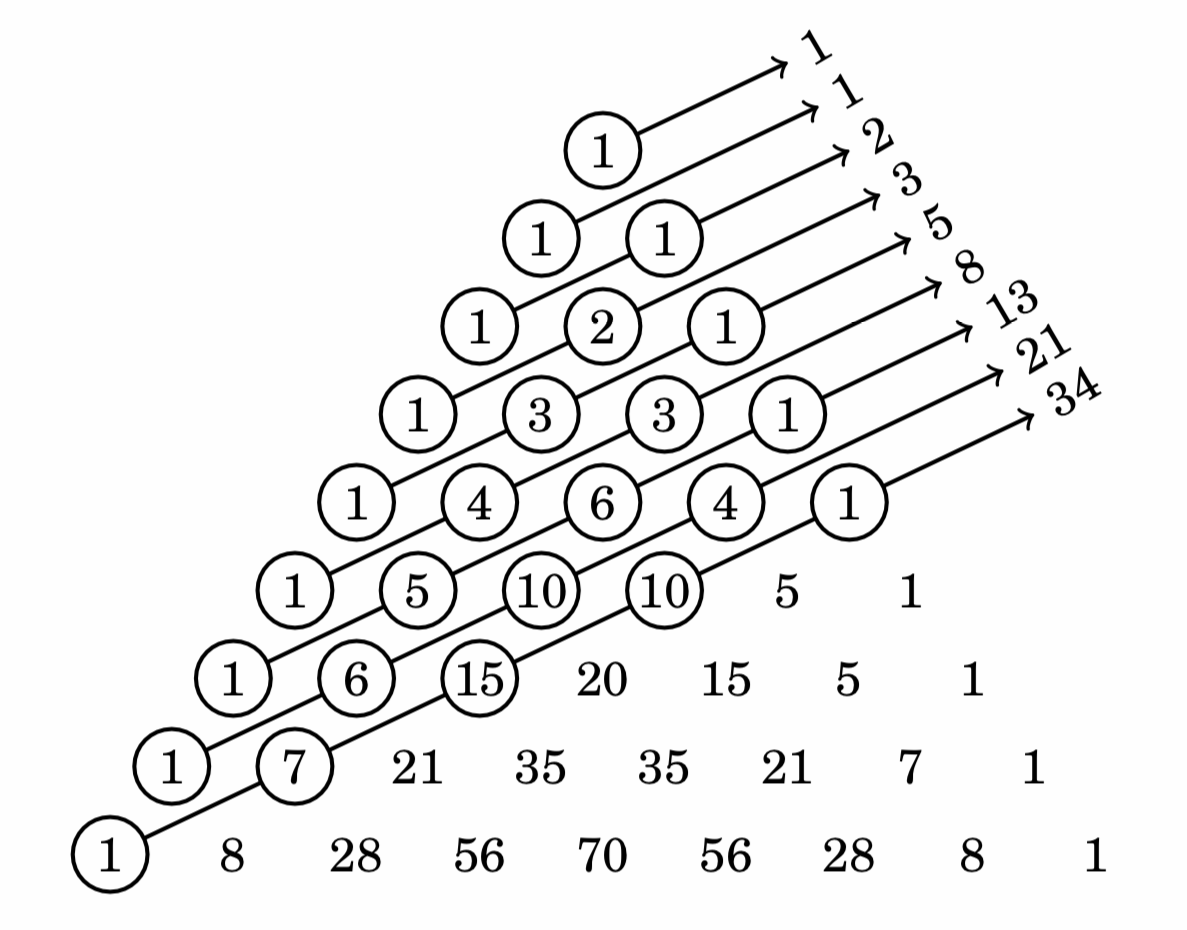
\includegraphics[width=.6\textwidth]{Pascaldiagonal}

\begin{solution}\\
Prove by induction that $\sum_{i=0}^n \binom{n-i}{i} = F_n$.\\

Base cases:

$n=0$: $\sum_{i=0}^0 \binom{-i}{i} = 1 = F_0$

$n=1$: $\sum_{i=0}^1 \binom{1-i}{i} = \binom{1}{0} + \binom{0}{1} = 1 = F_1$\\

Inductive step:

Assume by strong induction that $\sum_{i=0}^j \binom{j-i}{i} = F_j$ for $0 \le j \le k$.

\begin{align*}
    \sum_{i=0}^k \binom{k-i}{i} &= F_k\\
    \sum_{i=0}^k \binom{k-i}{i} + \sum_{i=0}^{k-1} \binom{k-1-i}{i} &= F_k + F_{k-1}\\
    \sum_{i=0}^k \binom{k-i}{i} + \sum_{i=1}^{k} \binom{k-i}{i-1} &= F_{k+1}\\
    \sum_{i=0}^k \binom{k-i}{i} + \sum_{i=0}^{k} \binom{k-i}{i-1} &= F_{k+1}\\
    \sum_{i=0}^k (\binom{k-i}{i} + \binom{k-i}{i-1}) &= F_{k+1}\\
    \sum_{i=0}^k \binom{k+1-i}{i} &= F_{k+1}\\
    \sum_{i=0}^{k+1} \binom{k+1-i}{i} &= F_{k+1} \qquad \text{since } \binom{k+1 - (k+1)}{k+1} = 0\\
\end{align*}

Then by strong induction we have that $\sum_{i=0}^n \binom{n-i}{i} = F_n$.
\end{solution}


\end{questions}
\end{document}
